\section{Results and discussion}\label{sec:discussion}
Though limited in the amount of involved people and performances, the experiments described in the previous section were helpful to start the discussion about the pedagogical applications of NMPs with musicians, and to collect useful comments and suggestions that will guide our investigation. 

\subsection{Objective, subjective and biological metrics}
In the two experiments, we investigate the sense of presence and quality of performance of the couple of subjects in case of visual occlusion (co-presence experiment) and different network latency conditions (networked performance). The acquisition and evaluation was performed using subjective and objective metrics \cite{CIM2018}. 

With regard to the former, we used a post-experiment 27-item questionnaire divided in five main topics, such as \textit{Predictability and Interaction}, or \textit{Quality of the Music Performance}. After each phase of the networked experiments, we asked a subset of five questions to evaluate the impact of different latency conditions in the questionnaire.

With regard to the latter, we acquired the audio recordings of the networked performance, manually tracked the beat, extracted a BPM trend and computed a degree of acceleration/deceleration from it. Other metrics used in NMP literature include the pacing, the regularity or the asymmetry of the performance \cite{RottondiOverview}.



an objective metrics computed from the audio acquisition related to the degree of acceleration or deceleration of the performance . The latter is one of the metrics
 

\begin{figure}[t]
	\centering
	\begin{subfigure}[t]{.48\columnwidth}
		\centering        
		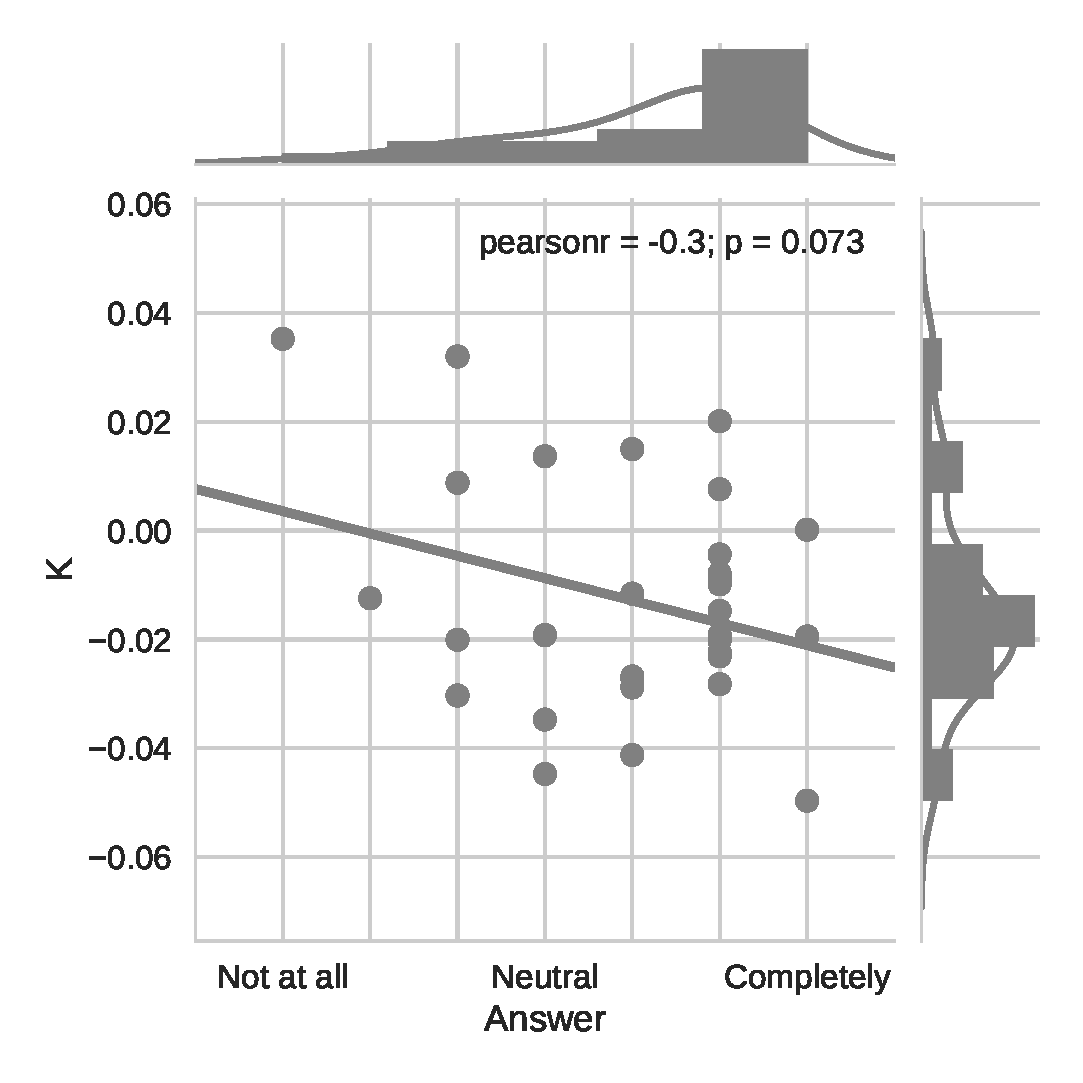
\includegraphics[trim={0cm 0cm 1cm 0cm},clip,width=\textwidth]{img/compelling}
		\caption{Influence of the visual feedback}
		\label{subfig:compelling}
	\end{subfigure}
	\begin{subfigure}[t]{.48\columnwidth}
		\centering        
		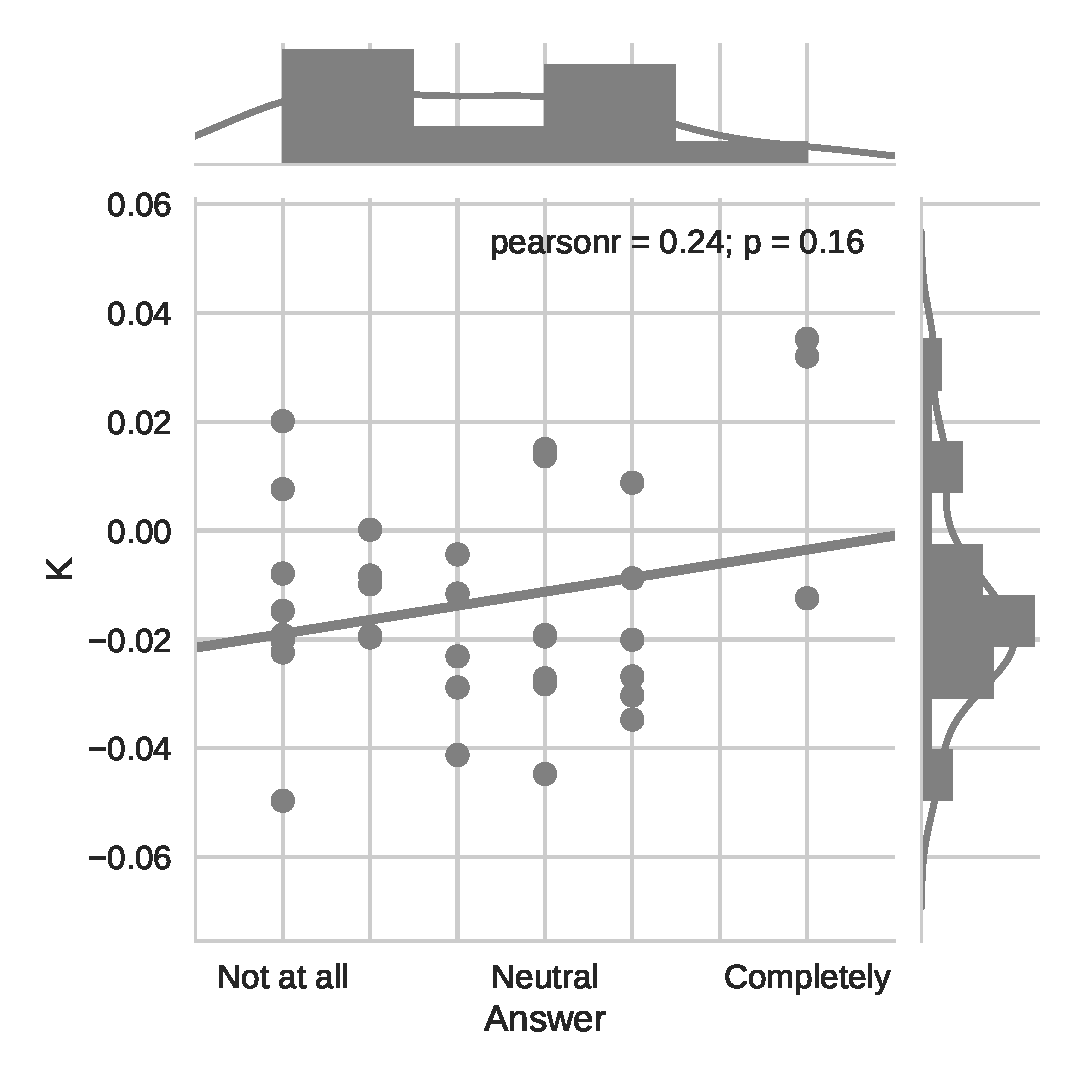
\includegraphics[trim={1.5cm 0cm 0cm 0cm},clip,width=\textwidth]{img/involvement}
		\caption{Influence of the auditory feedback}
		\label{subfig:involvement}
	\end{subfigure}
	\quad 
	\caption{Histogram of the answers on the influence of visual and auditory feedback after the NMP experiment.}\label{fig:ca}
	%	\vspace{-1em}
\end{figure}  


\subsection{Auditory and visual feedback}
From the first experiment, we could observe different strategies of musical coordination and interpretation, based on breathing signaling and communicative gestures to keep synchronization, especially for attacks and the duration of sustained notes. In this case, the no sight condition deeply affected the expressiveness of the performance. In full visual occlusion, the performers relied mostly on acoustic cues to keep the tempo, with the apparent effect of an acceleration during the performance. 

This aspect is also investigated in the remote performance by asking in the perceptual questionnaire how much the visual and auditory display quality interfered or distracted them from performing. In Figure \ref{fig:va} we display a histogram of the answers in a 7-point likert scale. While the influence of the visual feedback is limited (Fig \ref{subfig:visual}), the auditory feedback is predominant for the performance.
  
  
\begin{figure}[t]
	\centering
	\begin{subfigure}[t]{.48\columnwidth}
		\centering        
		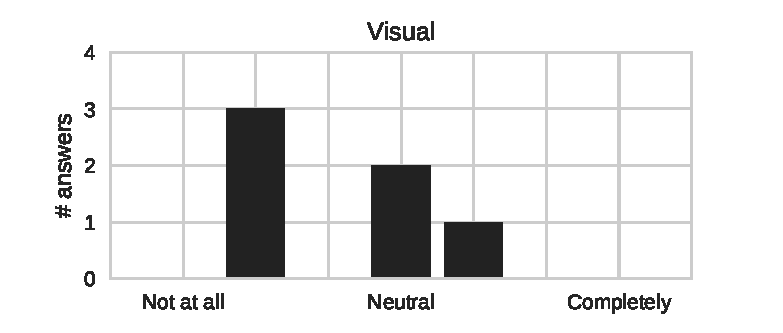
\includegraphics[trim={.5cm 0cm 1cm 0cm},clip,width=\textwidth]{img/Visual}
		\caption{Influence of the visual feedback}
		\label{subfig:visual}
	\end{subfigure}
	\begin{subfigure}[t]{.48\columnwidth}
	\centering        
	\includegraphics[trim={1.5cm 0cm 0cm 0cm},clip,width=\textwidth]{img/Audio}
	\caption{Influence of the auditory feedback}
	\label{subfig:audio}
\end{subfigure}
	\quad 
	\caption{Histogram of the answers on the influence of visual and auditory feedback after the NMP experiment.}\label{fig:va}
%	\vspace{-1em}
\end{figure}  
  
\subsection{Peripherical visual feedback}
The partial occlusion condition somewhat mimics a possible strategy for visual information reduction in remote performance (blob). 


\subsection{Mono vs Stereo vs 3D Audio}

\subsection{Environment: matching acoustics}

\subsection{Measure for latency compensation and virtual conductor}

